\subsection{Decision Trees}
\label{sub:DT}

% Introduction & Building Blocks
A \gls{dt} is a non-parametric supervised learning algorithm used for both classification and regression tasks. It has a hierarchical, tree-like structure consisting of a root node, branches, internal nodes and leaf nodes, as shown in figure \ref{fig:decision_tree}.

\begin{figure}[ht]
    \centering
    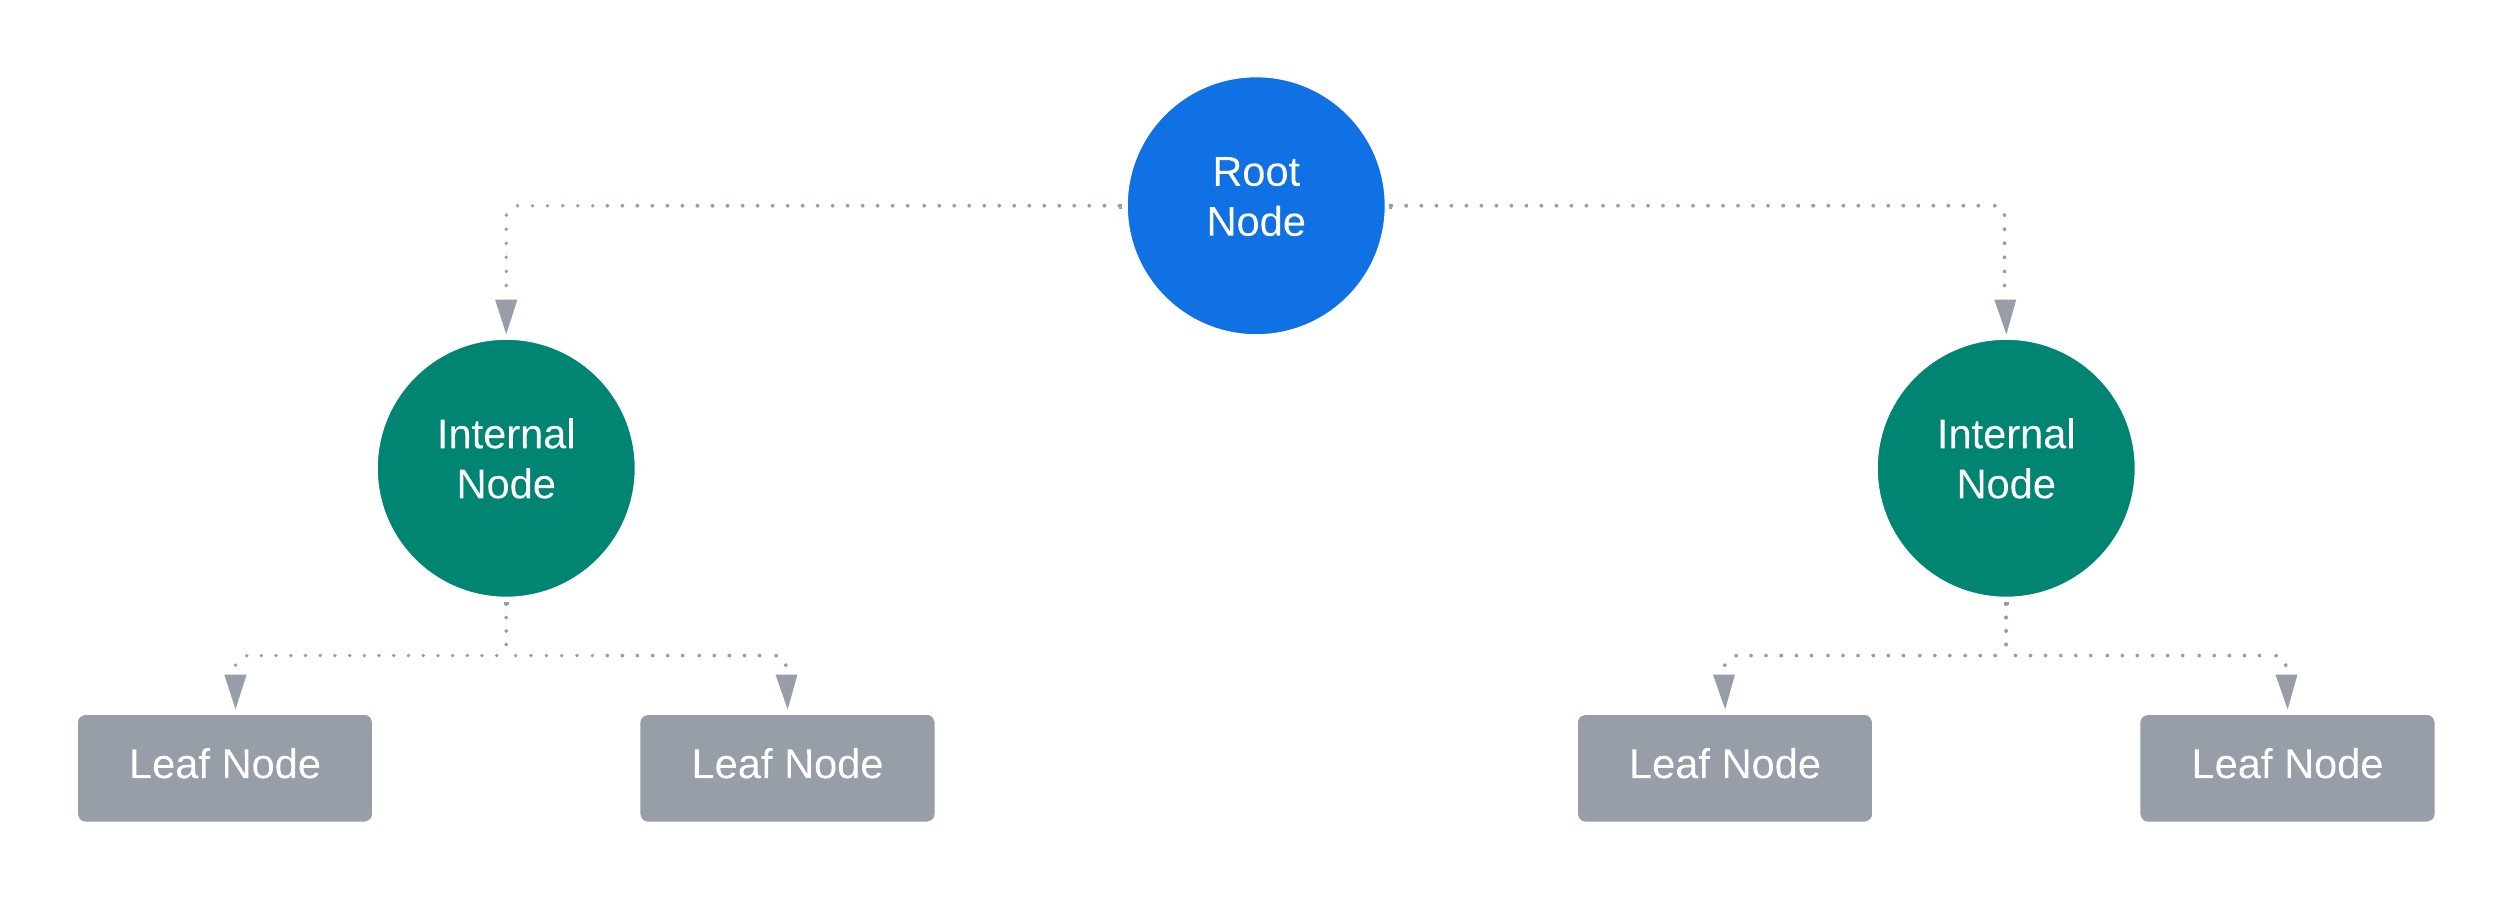
\includegraphics[width=0.75\textwidth]{./assets/img/decision_tree.png}
    \caption{At the top is the root node with no incoming branches. Branches then extend from the root node to reach internal nodes. Further branches then extend from the internal nodes to the leaf nodes. These leaf nodes contain all the possible outcomes within the dataset.}
    \label{fig:decision_tree}
\end{figure}

\noindent
% Learning Process
In the learning process, \glspl{dt} use a divide-and-conquer strategy. They perform a greedy search to find optimal splitting points within the tree. This splitting process occurs in a top-down, recursive manner until all or most of the data points have been assigned a specific class label. Whether all data points are classified into homogeneous sets depends on the complexity of the tree. Smaller trees tend to reach pure leaf nodes, where data points belong to a single class, as illustrated in figure \ref{fig:pure_leaf_node}. However, as trees grow larger, it becomes difficult to maintain purity, often resulting in data fragmentation. This fragmentation, known as overfitting, occurs when too little data falls within a subtree.

\begin{figure}[ht]
    \centering
    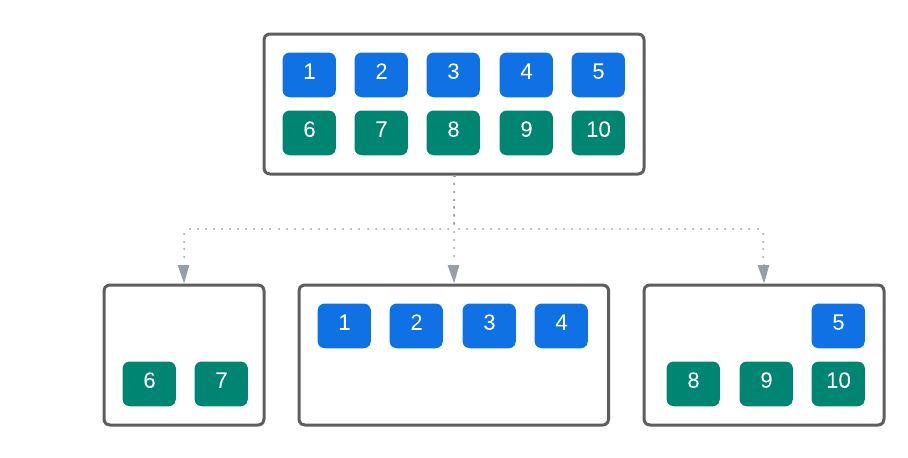
\includegraphics[width=0.75\textwidth]{./assets/img/pure_leaf_node.png}
    \caption{Illustration of a \gls{dt} with two pure leaf nodes on the left and in the middle.}
    \label{fig:pure_leaf_node}
\end{figure}

\noindent
% CART Algorithm
A commonly used algorithm for building \glspl{dt} is the \gls{cart} algorithm introduced by \cite{breiman1984classification}. The \gls{cart} algorithm is widely used to construct decision trees for both classification and regression tasks.
\newline
\newline
\gls{cart} constructs \glspl{dt} through a recursive binary partitioning process. Given a data set $D$ with features $x$ and a target variable $y$, the algorithm aims to partition the data set into subsets $D_1$ and $D_2$ based on a selected feature $x_i$ and a threshold $\theta$ such that

\begin{align*}
    D_1 &= \{ (x, y) \in D \,|\, x_i \leq \theta \} \\
    D_2 &= \{ (x, y) \in D \,|\, x_i > \theta \}
\end{align*}

\noindent
The goal is to identify optimal splits that maximise the purity of the resulting subsets. For classification tasks, purity is often measured by metrics such as Gini impurity, and for regression tasks it may include metrics such as \gls{mse}. The algorithm applies this splitting process recursively to subsets until a stopping criterion is met, such as reaching a predefined depth or having too few data points in a node.
\newline
\newline
% Pruning to reduce complexity
To reduce overfitting and produce more interpretable models, \glspl{dt} favour smaller trees. Complexity reduction is usually achieved through a process called pruning. Pruning selectively removes branches that split on less important features, resulting in simpler and more generalised trees.
\newline
\newline
% Ensembling Methods
To mitigate the problem of overfitting and improve prediction accuracy, \glspl{dt} can be combined using ensemble methods rather than relying on individual trees alone. Ensemble methods combine the outputs of multiple \glspl{dt}, called weak learners. Two prominent ensemble methods are bagging and boosting.

% Bagging (bootstrap aggregation)
\subsubsection{Bagging}
\label{subsub:bagging}
In bagging, a large number of individual weak learners independently make predictions for the target variable. The ensemble then consolidates these predictions through a consensus mechanism. For classification tasks, this is often a majority vote, where the most frequently predicted class among the trees is selected. For regression tasks, a weighted average of the predictions is computed.

% Boosting
\subsubsection{Boosting}
\label{subsub:boosting}
Boosting combines weak learners sequentially, typically in the form of \glspl{dt} with only one split, called \textit{decision stumps}. The sequential nature of boosting allows each new learner to correct the errors of its predecessors, leading to improved prediction accuracy. Boosting produces predictions for both classification and regression tasks by a weighted combination of the outputs of multiple weak learners.
\newline
\newline
In classification tasks, boosting begins by training a base classifier, typically a weak learner, on the original dataset. Misclassified data points from the initial classifier are then given higher weights, while correctly classified data points are given lower weights. This weighting emphasises the importance of the data points that challenge the capabilities of the current classifier. Subsequent weak learners are trained sequentially to refine the predictions, with each new learner focuing on correcting the errors made by the ensemble up to that point. When making predictions, all the weak learners contribute weighted votes, with better performing classifiers receiving higher weights. The final prediction is determined by combining these weighted votes.
\newline
\newline
For regression tasks, boosting also starts with a weak regressor as the base model. Instead of modelling the target variable directly, boosting focuses on modelling the residuals or errors produced by the ensemble of weak regressors. The first weak regressor is trained to predict these residuals. Similarly, subsequent weak regressors are added sequentially to further improve the predictions. To make final predictions, the outputs of these weak regressors are aggregated by summing their contributions.